\section{Lecture 2: Gradient Descent}
\sectionlabel{gradient_descent}

\subsection{Gradient Descent}

% TODO: Gradient descent figure?

The procedure of gradient descent is defined by the recursion:
\[
x_{t+1} = x_t - \eta \nabla f(x_t)
\]
where $\eta$ is the step size. This works to solve the problem
\[
\min_{x\in\domain} f(x)
\]
for $f$ convex, differentiable, and L-Lipschitz

\begin{definition}[L-Lipschitz]
A function is said to be \emph{L-Lipschitz} if its gradient is bounded,
\[
\|\nabla f(x)\| \leq L
\]
\end{definition}

\begin{fact}
f(x) is L-Lipschitz implies that the difference between two points in the range is bounded,
\[
|f(x) - f(y)| \leq L \|x - y\|
\]
\end{fact}

\begin{question}
How do we ensure that $x_{t+1}\in\domain$?
\end{question}

Solution: Project onto $\domain$

\begin{definition}[Projection]
The \emph{projection} of a point $y$ onto a set $\domain$ is defined as
\[
\Pi_{\domain}(x) = \argmin_{y\in\domain} \|x-y\|
\]
\end{definition}

\begin{example}
\examplelabel{euclidean-ball}
A projection onto the Euclidean ball $B_2$ is just normalization:
\[
\Pi_{B_2}(x) = \dfrac{x}{\|x\|}
\]
\end{example}

\begin{figure}
\figurelabel{project}
\begin{center}
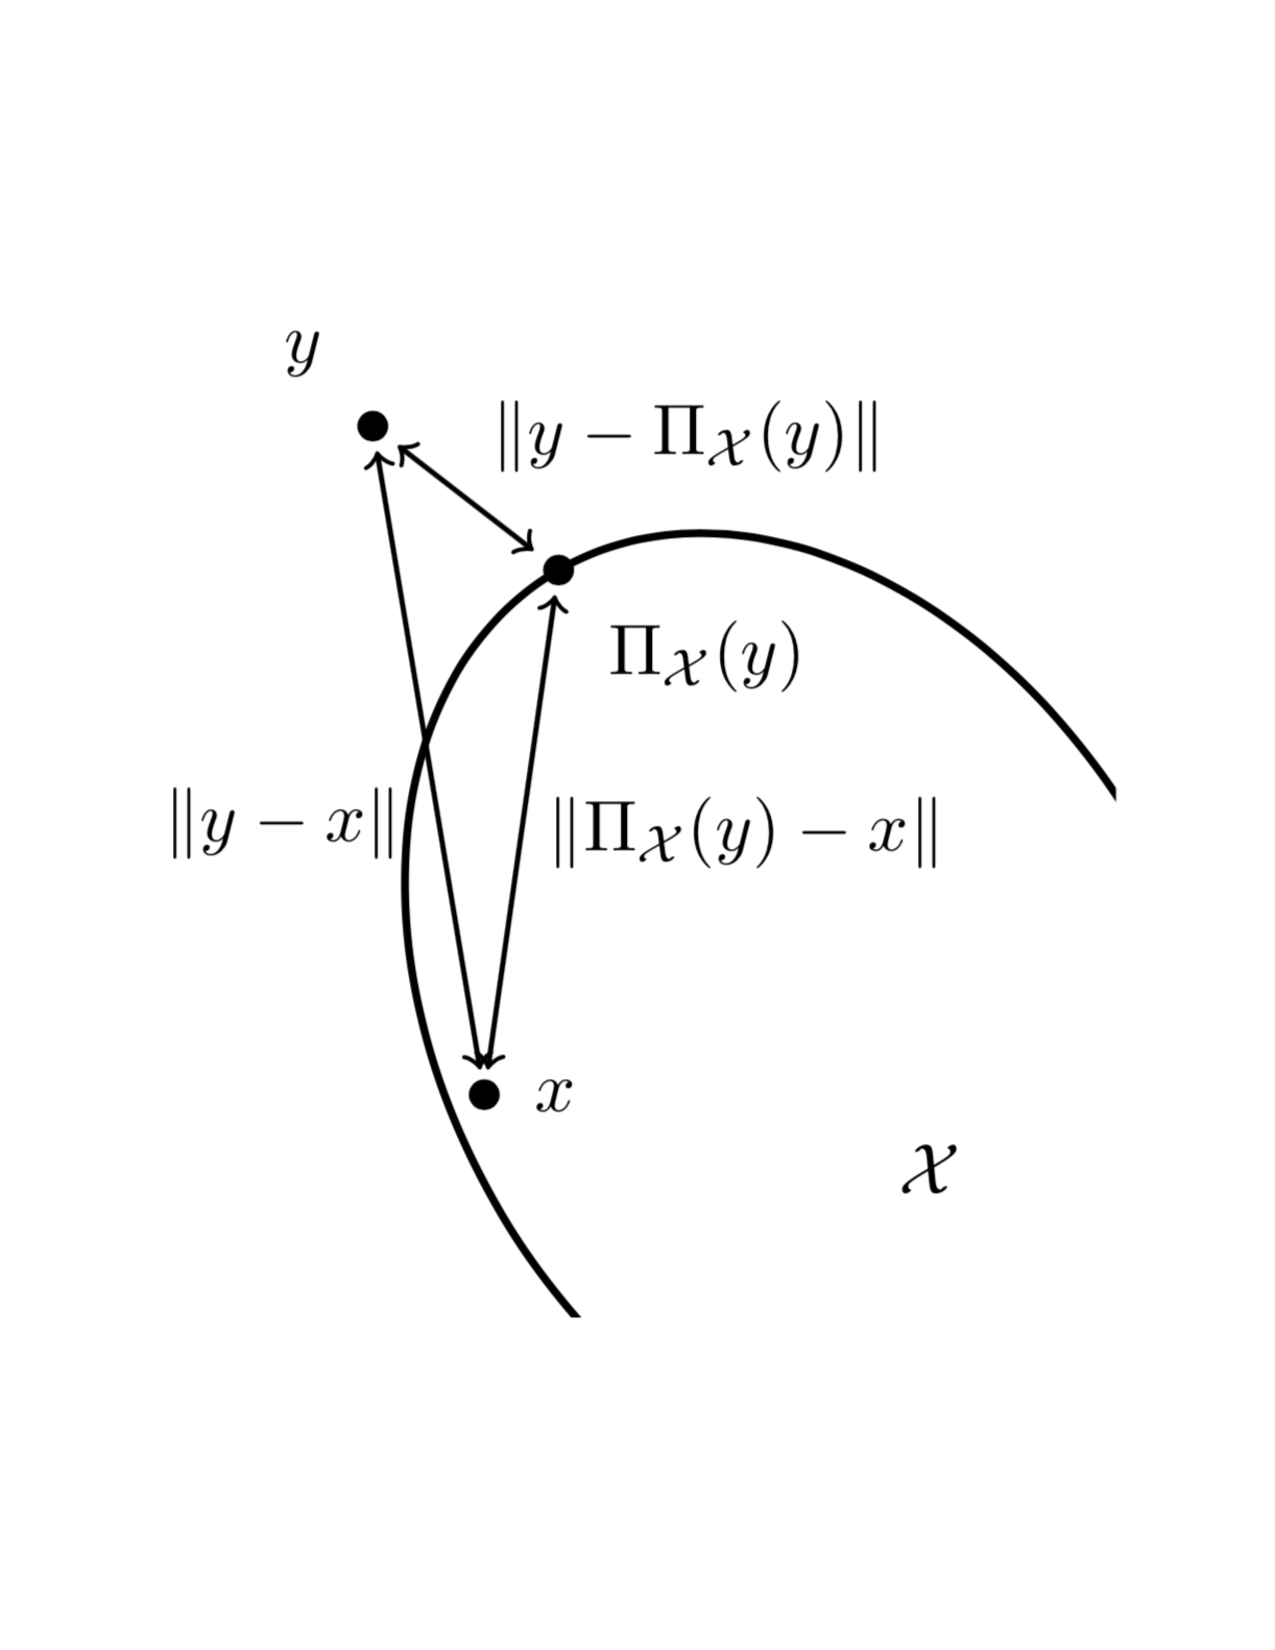
\includegraphics[width=3in]{figures/lecture2-projection}
\end{center}
\caption{Projection of $y$ onto set $\mathcal{X}$. }
\end{figure}

%TODO Indentation
The crucial property of projections is that they satisfy the following condition:
\[
\| \Pi_{\domain}(y) - x \|^2 \leq \| y - x \|^2
\]
i.e. the projection of $y$ onto a convex set containing $x$ is closer to $x$. See \figureref{project} for a geometric picture.

\begin{lemma}
\[
\| \Pi_{\domain}(y) - x \|^2 \leq \| y - x \|^2 - \| y - \Pi_{\domain}(y) \|^2
\]
Which follows from the Pythagorean theorem. Note that this lemma implies the above property.
\end{lemma}

\subsubsection{Modifying Gradient Descent with Projections}

So now we can modify our original procedure to use two steps.
\[
y_{t+1} = x_t - \eta \nabla f(x_t)
\]
\[
x_{t+1} = \Pi_{\domain}(y_{t+1})
\]

And we are guaranteed that $x_{t+1}\in\domain$. Note that computing the projection may be the hardest part of your problem, as you are computing an $\argmin$. However, there are convex sets for which we know explicitly how to compute the projection (see \exampleref{euclidean-ball}).


\begin{theorem}[Project Gradient Descent for Lipchitz Functions]
\theoremlabel{libpchitz}
Assume that function $f$ is convex, differntiable, and closed with bounded gradients. Let $L$ be the Lipchitz constant of $f$ over the convex domain $\Omega$. Let $R$ be the upper bound on the distance from the initial point $x_1$ to the optimal point $x^* = \arg\min_{x \in \Omega} f(x)$ (i.e. $\lVert x_1 - x^* \rVert_2$). Let $t$ be the number of iterations of project gradient descent.

If the learning rate $\eta$ is set to $\eta=\frac{R}{L \sqrt(t)}$, then $f\left(\frac{1}{t}\sum_{s=1}^t x_s\right) - f\left(x^*\right) \leq \frac{RL}{\sqrt{t}}$.

This means that the difference between the functional value of the average point during the optimization process from the optimal value is bounded above by a constant proportional to $\frac{1}{\sqrt{t}}$.

\end{theorem}

Before proving the theorem, recall that
\begin{itemize}
    \item First order characterization of convexity: $f(y) = f(x) + \nabla f(x)^\top (y - x)$
    \item "Fundamental Theorem of Optimization": An inner product can be written as a sum of norms: $u^\top v = \frac{1}{2}(\lVert u \rVert^2 + \lVert v \lVert^2 - \lVert u - v \rVert^2$. This property can be seen by writing $\lVert u - v \rVert$ as $\lVert u - v \rVert = \lVert u \rVert^2 + \lVert v \lVert^2 - 2 u^\top v$.
    \item $L$-Lipchitz: For all $x$, $\lVert \nabla f(x) \rVert \leq L$.
    \item $\lVert \pi_\Omega (y) - x \rVert^2 \leq \lVert y - x \rVert^2 - \lVert y - \pi_\Omega (x) \rVert^2$ % From above TODO
\end{itemize}


\begin{proof}[Proof of \theoremref{libpchitz} for compact sets.]
The proof begins by first bounding the difference in function values $f(x_s) - f(x^*)$.
\begin{align}
    f(x_s) - f(x^*) \leq
\end{align}
\end{proof}
